\section{Trend and business cycle: long-run stylised facts}

\section{The Solow-Swan model}\label{solow-swan-model}
\subsection*{General assumptions}
\begin{enumerate}
    \item A closed economy
    \item No Government, thus we do not have to consider taxes and all income is available for consumption
\end{enumerate}

\textbf{Assumes a Neoclassical production function:}
\begin{equation}\label{production_function}
Y(t)=F\left[B(t)K(t), A(t)L(t)\right]
\end{equation}
 where
 \begin{align*}
 \frac{\partial F}{\partial (B,K)}>0
 &&
 \frac{\partial F}{\partial (A,L)}>0
 \end{align*}

We are familiar with this production function and its inputs. $B$ and $A$ represent effectiveness of capital and labor respectively. 

The production function \ref{production_function} has a few mathematical characteristics:
\begin{itemize}
\item
  It is a positive function, i.e.~the output cannot be negative
\item
  To simplify we assume that the function is continuous and
  twice-differentiable
\item
  Marginal productivity is positive
\item
  Returns to scale are constant
  \begin{itemize}
  \item The economy is big enough to have exhausted the gains from specialization
  \item In a small economy we can expect "more than double" increase in output with specialization (Economies of Scale i.e.)
  \end{itemize}
  \item Inputs other than capital, labour and knowledge are not important, such as land other natural resources. 
\item
  The model satisfies the Inada-conditions
 
\begin{align*}
\lim_{B * K \rightarrow 0 } \frac{\partial F}{\partial (B,K)}= \infty   
&&
\lim_{A * L \rightarrow 0 } \frac{\partial F}{\partial (A,L)}= \infty
\end{align*}

\begin{align*}
\lim_{B * K \rightarrow \infty } \frac{\partial F}{\partial (B,K)}= 0    
&&
\lim_{A * L \rightarrow \infty } \frac{\partial F}{\partial (A,L)}= 0
\end{align*}

  \begin{itemize}
  \item
    In economic terms it says that marginal product of capital is very large when the capital stock is sufficiently small and that it becomes smaller when capital grows. Imagine an economy with $K(0)$; it will not have any output. When we introduce a little bit of capital, the marginal product of that initial capital is very high. 
  \end{itemize}
\end{itemize}

\subsubsection*{Production Functions with different forms of technical progress}
The model can use technical progress, we have have a few different types of technical progress. It is useful to notice that such progress can be both tangible and intangible. An example is how the increased hand-hygiene in hospitals significantly reduced the amount of hospital related deaths. 

\subsubsection*{Capital Augmenting technical progress}
\begin{align}
A(t) = 1 \implies Y(t)=F\left[B(t)K(t),L(t)\right]
\end{align}
The equation shows that labor cannot get more productive. 

\subsubsection*{Factor Augmenting technical progress}
\begin{align}
A(t) = 1 \implies Y(t)=F\left[B(t)K(t),L(t)\right]
\end{align}

\subsubsection*{Labour Augmenting technical progress}
\begin{align}
B(t) = 1 \implies Y(t)=F\left[K(t),A(t)L(t)\right]
\end{align}
The equation shows that capital cannot get more productive. 

\subsubsection{The Solow-Swan model on intensive form}
Output only changes over time, $t$ if the inputs $(K, L, A)$ change. More specifically we need an increase in A, knowledge, to increase the output of capital and labor over time.
To simplify we can omit time from the production function. 


The empirical data showed us that the Labor Augmenting production function seems to be more correct.

Intensive form means that we look at the production function in terms of effective labor. 
\subsubsection*{The Production Function}
\begin{equation}
Y=F(K,AL)
\end{equation}
Since we are assuming that we have constant returns to scale on inputs K and AL, we can rewrite the production function on the intensive form, which means we look at output and capital input in terms of effective labor. We divide by AL.

\begin{equation*}
\frac{Y}{AL}=\frac{F(K,AL)}{AL}\implies\frac{Y}{AL}=F(\frac{K}{AL},1)
\end{equation*}

Now we define $\frac{Y}{AL}$ as \textit{y} which is output per unit of effective labor and $\frac{K}{AL}$ as \textit{k} which is capital per unit of effective labor. We also define $F(\frac{K}{AL},1)$ as \textit{f(k)}. We can then rewrite the production function like this:

\begin{equation}\label{production_intensive}
y=f(k)
\end{equation}

This now shows us that the output per unit of effective labour is a function of capital per unit of effective labor. 

\begin{quotation}
To see the intuition behind \ref{production_intensive}, think of dividing the economy into $AL$ small economies, each with 1 unit of effective labor and $K/AL$ units of capital. Since the production function has constant returns, each of these small economies produces $1/AL$ as much as is produced in the large, undivided economy. Thus the amount of output per unit of effective labor depends only on the quantity of capital per unit of effective labor, and not on the over- all size of the economy. This is expressed mathematically in equation \ref{production_intensive}. \textcite{romer_advanced_2012}[pp. 11]
\end{quotation}

Furthermore the \textit{f(k)} is assumed to satisfy: $f(0)=0, f'(k)>0, f''(k) > 0$. Which means that it is a positive function with a maximum. 

\begin{quotation}
Since $F(K,AL)$ equals $AL \cdot f (K/AL)$, it follows that the marginal product of capital, $\partial F(K,AL)/ \partial K$ equals $ALf'(K/AL)(1/AL)$, which is just $f '(k)$. Thus the assumptions that $f '(k)$ is positive and $f ''(k)$ is negative imply that the marginal product of capital is positive, but that it declines as capital (per unit of effective labor) rises. \textcite{romer_advanced_2012}[p. 12]
\end{quotation}

\subsubsection*{The Evolution of inputs over time}
\begin{equation*}
L(t)=L(0)*e^{nt}
\end{equation*}

$L(t)$ is the workforce in any period t. $L(0)$ represents the initial workforce. So the total workforce evolution depends on it's initial level times an exponential function of time - $t$ - and the exogenous rate of growth of the population - $n$.

\begin{align*}
A(t)=A(0)*e^{gt} ,&& g>0
\end{align*}

$A(t)$ represents the knowledge as a production input in the economy over time. As with $L(t)$ it varies depending on the initial level of knowledge $A(0)$, times an exponential function of time - $t$ - and the exogenous rate of technical progress - $g$.

Both technical progress ($A(t)$) and the workforce ($L(t)$) grow exponentially over time. 

\begin{equation*}
    \dot{K}(t)=s*Y(t)-\delta*K(t)
\end{equation*}

This equation gives us evolution of capital over time, and it depends on the savings rate times total production for the same period and and an exogenous rate of depreciation - $\delta$ - times the capital stock. In the long run, since we have no government and a closed economy all savings are invested, therefore we can simplify by defining: $sY(t) = I(t) $.

\subsubsection*{The Consumption Function}
\begin{equation}
C=(1-s)Y_d
\end{equation}
\begin{equation*}
\end{equation*}
We assume that the economy is closed and that we have no government, so disposable income is unaffected by taxes or trade, therefore we can write $Y_d=Y$. In the consumption function we have $s$ which is the marginal propensity to save and what isn't saved is consumed. 

\subsubsection*{Savings and Investment}
In the Solow growth model, the savings rate is an exogenous variable, and it is the variable that is most likely to be the target of policy changes. 

We defined investment as being equal to total savings

\begin{equation}
I = \dot{K} + \delta K
\end{equation}
 
\begin{figure}[H]
\centering
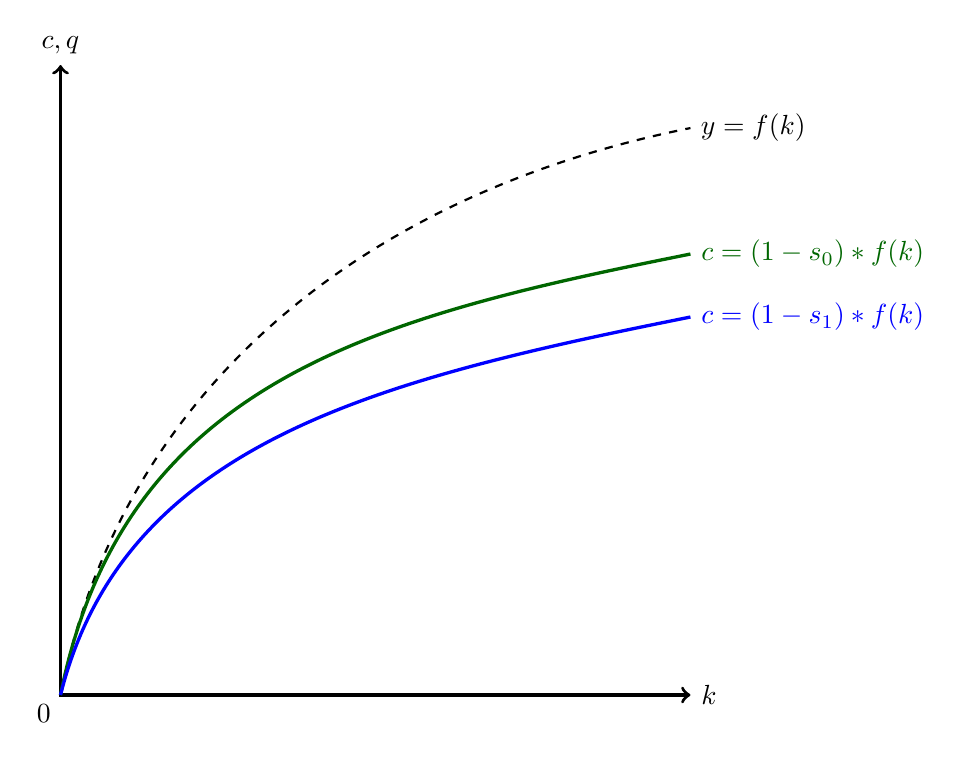
\begin{tikzpicture}[scale=0.8]\label{consumption_function_solow}
\draw[very thick,<->] (0,10) node[above]{$c,q$}--(0,0)--(10,0) node[right]{$k$};
\node [below left] at (0,0) {$0$};
\draw[dashed, thick] (0,0) ..controls (1,5) and (5,8) .. (10,9) node[right]{$y=f(k)$};
\draw[very thick, black!60!green] (0,0) ..controls (1,5) and (5,6) .. (10,7) node[right]{$c=(1-s_0)*f(k)$};
\draw [very thick, blue] (0,0) ..controls (1,4) and (5,5) .. (10,6) node[right]{$c=(1-s_1)*f(k)$};
\end{tikzpicture}
\caption{The Consumption Function the Solow Model and a change in the savings rate}
\end{figure}

Given consumption is a part of total production, the graph for consumption has the same shape as the production function. An increase of the savings rate will push the consumption function down - as $s_1 > s_0$.

\subsubsection*{The dynamics of $k$}
\begin{tcolorbox}[fontupper=\large, fontlower=\normalsize]
\begin{equation}\label{solow_fundamental}
    \dot{k}(t)=sf(k(t))-k(n+g+\delta)
\end{equation}
\tcblower
The Fundamental Equation of The Solow Model
\end{tcolorbox}

\ref{solow_fundamental} is what is refered to as the key equation of the Solow Model. $\dot{k}(t)$ is the growth rate of the capital stock per unit of effective labour, and it depends on the investment per unit of effective labour - $sf(k(t))$ - and the break even level of investment - $k(n+g+ \delta )$ - which is the minimum level of investment needed to maintain a constant level of $k$. Two reasons for this to be break even level of investment:
\begin{itemize}
    \item Existing capital is depreciating, and it must be replaced to keep the capital stock from falling, this is given by $\delta k$
    \item The quantity of effective labour is growing at rate $n+g$, thus keeping the investment constant is not enough to keep the capital stock per unit of effective labour constant, so capital stock must also grow by $n+g$
\end{itemize}
The following graph returns the relation described above:

\begin{figure}[H]
\centering
\begin{tikzpicture}[scale=0.8]
\draw[thick,<->] (0,10) node[above]{$\frac{I}{AL}$}--(0,0)--(10,0) node[right]{$k$};
\node [below left] at (0,0) {$0$};
\draw(0,0)--(9,9) node[right]{$(n+g+\delta) k$};
\draw(0,0) ..controls (1,5) and (5,6) .. (10,7) node[right]{$sf(k)$};
\draw[dashed] (6.1,6.1) -- (6.1,0) node[below]{$k^*$};
\end{tikzpicture}
\caption{Investment in the Solow Model}
\end{figure}

\begin{itemize}
    \item The 45\textdegree line $(n+g+ \delta)k$ represents the break-even level of investment.
    \item The curve $sf(k)$ represents total investment.
\end{itemize}

Given that the optimal level of investment $k^*$ is given by the interception between the two functions, $sf(k)=(n+g+ \delta)k \implies \dot{k}=0$.

\subsubsection{Steady State in the Solow Model (Balanced Growth Path)}

Recall equation \ref{solow_fundamental}, we can define steady state as the long run equilibrium where quantities grow at constant rates. In the Solow model's steady state, $k=k^{*}$. At $k^{*}$ the variables grow at constant rates: 
\begin{itemize}
    \item Labour grows at rate $n$;
    \item Technical progress grows at rate $g$;
    \item Because $K=ALk$, K grows at rate $n+g$;
    \item Since we assume constant returns to scale, $y=f(k)$, will grow at the same rate as $k$, which is the same as the growth rate of $K$, which will be $n+g$;
    \item Output per worker, $\frac{Y}{L}$, and capital per worker, $\frac{K}{L}$, are both growing at the constant rate $g$.
\end{itemize}




\subsubsection*{The Golden Rule of Capital Accumulation}
The Golden Rule of Capital Accumulation ensures that the level of consumption is maxmimized. There exists a level of the savings rate, which maximizes the consumption, denoted as $s_\text{gold}$. The savings rate that reaches this level corresponds to a capital accumulation level $k_\text{gold}$. At $k_\text{gold}$ the capital accumulated is just enough to keep the capital stock constant after depreciation has been subtracted. Thus:

$$f'(k_\text{gold}) = \delta + n + g $$

If we are below $k_\text{gold}$, we can both save more and increase consumption at the steady state, and if we are above we can save less and still increase consumption at the steady state. 

With a Cobb-Douglas production function, the savings rate at the optimal level is $\alpha$. Because $s_{\text{gold}}$ is expressed as:

$$
s_{\text{gold}} = \frac{\text{MPK}}{APK}
$$

\subsubsection*{Dynamic inefficiency}
\begin{itemize}
    \item When the economy is below $k^*_\text{gold}$ , higher saving will increase consumption; when it is above $k^*_\text{gold}$, steady-state consumption can be increased by saving less.
    \item In the latter case, capital-labor ratio is too high so that individuals are investing too much and not consuming enough (dynamic inefficiency).
    
\item  Such dynamic inefficiency will not arise once we endogenous consumption-saving decisions. (Ramsey)
\end{itemize}
\subsubsection{Primary conclusions of the Solow Model}
\begin{enumerate}[i]
\item Simple and tractable framework, which allows us to discuss capital accumulation and the implications of technological progress
  \item Steady state is reached when the growth in the capital stock is just enough to keep the kapital stock per unit of effective labour constant. 
  \item Savings rate $s$ is exogenous and thus dynamic inefficiency can exist.
  \item No sustained growth without technological progress, which in the Solow model is exogenous $g_A$.
  \item Capital accumulation: determined by the saving rate, the depreciation rate and the rate of population growth. All are exogenous
  \item Differences in capital does not sufficiently explain cross-country income differences. 
\end{enumerate}


\begin{figure}
    \centering
    \includegraphics{1_0_Growth_Theory/solow_graphs.pdf}
    \caption{Output investment and consumption along the balanced growth path}
    \label{fig:my_label}
\end{figure}




